
\clearpage
\section{Customer Relationship Management}

Das CRM (Customer Relationship Management) ermöglicht Ihnen effizient Veranstaltungen (Anlässe, Präsentationen und Schulungen) zu koordinieren. Es unterstützt Sie bei der Einladung, dem Verwalten von Anmeldungen, Versenden von Erinnerungen und dem Erstellen von Teilnehmerlisten.

\vspace{\baselineskip}

Für Ihre Veranstaltung erstellen Sie bequem über eine Webseite eine Einladung, in Form eines Online-Flyers mit den wichtigsten Angaben zum Anlass, Eckdaten wie Termin, Zeit, Bemerkungen und Weiteres. Sie versenden an eine gewünschte Gruppe aus dem CRM eine Einladung, welche auf diese Einladungsseite verweist. Die Eingeladenen könne über diese Webseite Ihre Anmeldung am Anlass durchführen (mittels Klick) oder falls notwendig zu Beginn oder Später Ihre Entschuldigung einreichen. Sie als Organisator haben jederzeit den Überblick über die versendeten Einladungen und deren Status. Sie siehen sofort, wie viele Personen sich bereits an- oder abgemeldet haben. \\

Schliesslich können Sie sich eine Teilnehmerliste exportieren lassen und können auf diese Weise das Resultat Ihrer Einladung auswerten oder weiterreichen.

\vspace{\baselineskip}

Das CRM ist in zwei Teile gegliedert: 
\begin{itemize}
\item
\textbf{Veranstaltungstypen:} Hier legen Sie die verschiedenen Arten von Veranstaltungen fest (bspw. Jahresrückblick, Neuheiten-Präsentation etc.)
\item
\textbf{Veranstaltungen:} Unter diesem Menüpunkt werden die konkreten Veranstaltungen geplant. Nach dem Anlegen einer Veranstaltung haben Sie die Möglichkeit, die Einladungswebseite (Online-Flyer) zu gestalten.
\end{itemize}

\subsection{Veranstaltungstypen}

\textbf{Übersicht:} Klicken Sie im Menü links auf 'Customer Relationship Management' und den Unterpunkt Veranstaltungstypen. Die Übersicht der Veranstaltungstypen öffnet sich:

\begin{figure}[H]
\center{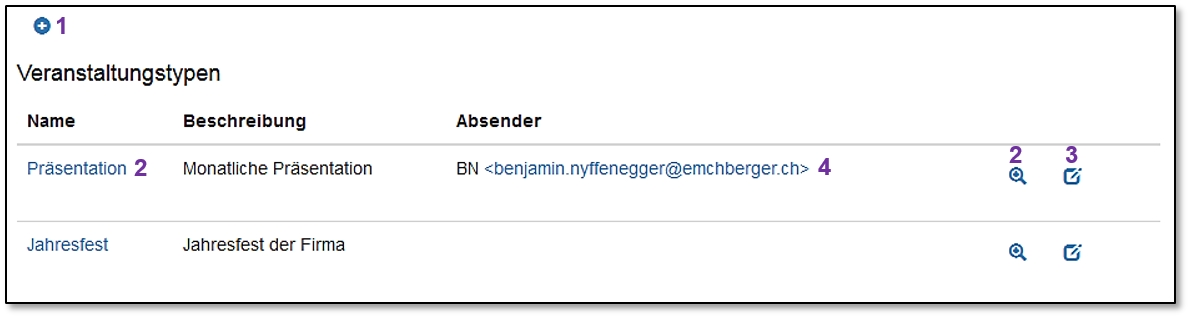
\includegraphics[width=1\linewidth]{../chapters/10_CRM/pictures/10-1_VeranstTyp_Uebersicht.jpg}}
\caption{Übersicht Veranstaltungstypen}
% \label{fig:speciation}
\end{figure}

Sie sehen alle erfassten Veranstaltungstypen. Mit Klick auf das Plussymbol 
\includegraphics[height=12pt]{/Icons/Plussymbol.jpg} \col{(1)} können Sie einen neuen Veranstaltungstyp erstelle. Mit Klick auf den entsprechenden Veranstaltungstyp \col{(2)} oder auf das Lupensymbol 
\includegraphics[height=12pt]{/Icons/Lupe.jpg} \col{(2)} können Sie die Details eines Veranstaltungstypen betrachten. Um einen Eintrag zu bearbeiten, klicken Sie auf das Bearbeiten-Symobol 
\includegraphics[height=12pt]{/Icons/Bearbeiten.jpg} \col{(3)}. Wurde eine Absender-Email-Adresse hinterlegt, können Sie mit Klick auf diese \col{(4)} eine Email versenden. Wählen Sie das gewünschte Emailprogramm aus.

\subsubsection{Neue Veranstaltungstypen anlegen}

\begin{figure}[H]
\center{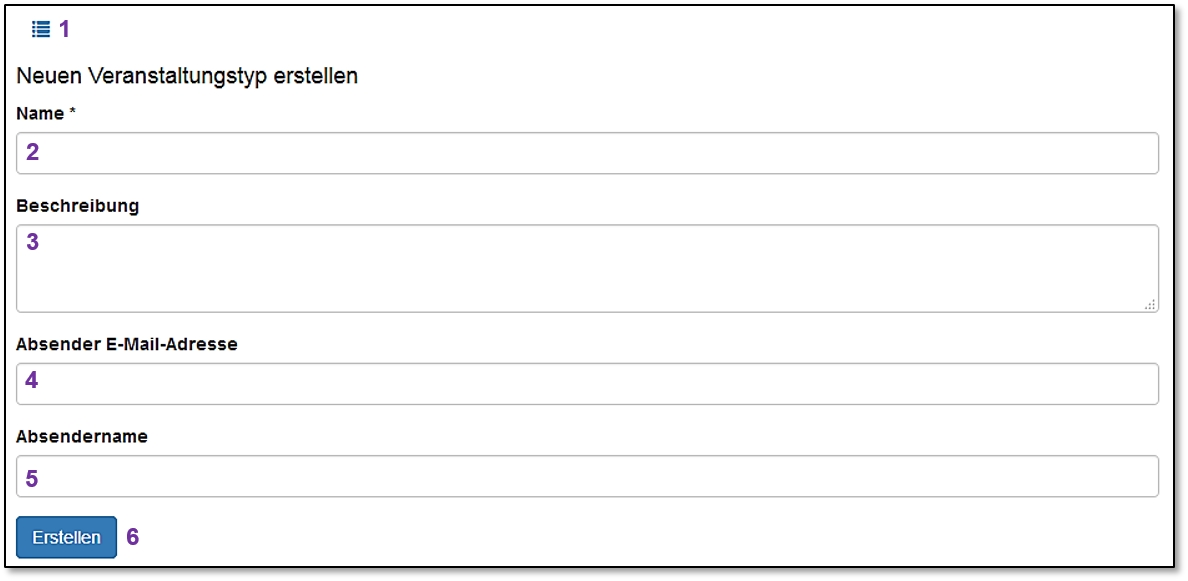
\includegraphics[width=1\linewidth]{../chapters/10_CRM/pictures/10-1_VeranstTyp_erstellen.jpg}}
\caption{Neue Veranstaltungstypen erstellen}
% \label{fig:speciation}
\end{figure}

Text x

\subsubsection{Bestehende Veranstaltungstypen betrachten und bearbeiten}

Text x

\vspace{\baselineskip}

\subsection{Veranstaltungen}

\textbf{Übersicht}

\begin{figure}[H]
\center{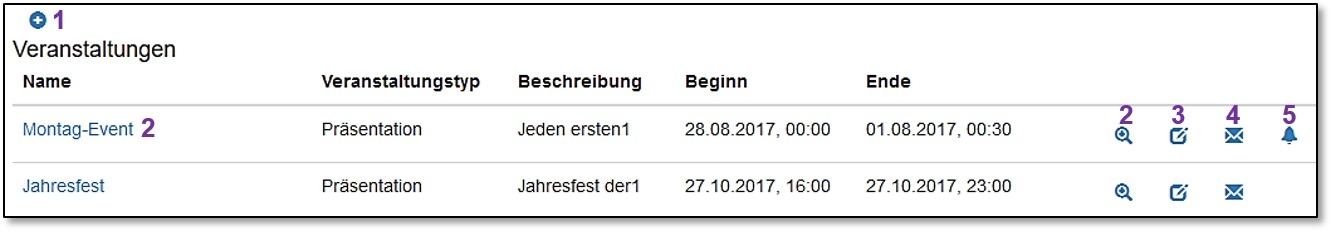
\includegraphics[width=1\linewidth]{../chapters/10_CRM/pictures/10-2_Veranstaltungen_Uebersicht.jpg}}
\caption{Übersicht Veranstaltungen}
% \label{fig:speciation}
\end{figure}

Text x

\subsubsection{Neue Veranstaltungen anlegen}

Text x

\subsubsection{Einladungsseite gestalten (Online-Flyer)}

Text x

\subsubsection{Teilnehmer verwalten}

inkl. Export
inkl. neue Person erfassen (Adressliste)
hinzufügen, löschen, Status ändern, 


\subsubsection{Einladungen versenden}

inkl. Emailvorlage bearbeiten

\subsubsection{Bestehende Veranstaltungen betrachten und bearbeiten}

Veranstaltung löschen
Text x

